\documentclass[referee,pdflatex,sn-mathphys-num]{sn-jnl}

\usepackage[T1]{fontenc}
\usepackage[utf8]{inputenc}
\usepackage{amsmath,amssymb,graphicx,longtable,booktabs,array,calc,xurl,xcolor,needspace}
\let\burl\url
\hypersetup{hidelinks,pdfauthor={Tivdzua Lubem Noah; Bader Rasheed; Dmitriy S. Vatolin}}
\raggedbottom

\begin{document}
\title[First-step faults and scheduler delay in Adam]{Separating First-Step Learning-Rate Faults from Scheduler Delay in Adam Training}

\author*[1]{Tivdzua Lubem Noah}\email{l.tivdzua@innopolis.university}
\author[1]{Bader Rasheed}\email{b.rasheed@innopolis.university}
\author[1]{Dmitriy S. Vatolin}\email{dmitriy@graphics.cs.msu.ru}
\affil[1]{\orgname{Innopolis University}, \orgaddress{\city{Innopolis}, \country{Russia}}}
\affil[]{ORCID (Tivdzua Lubem Noah): \href{https://orcid.org/0009-0009-2511-1800}{0009-0009-2511-1800}}
\abstract{\textbf{Purpose} Large early updates can harm neural-network training, but that fact does not distinguish a single incorrect update from continuing scheduler delay or inadequate subsequent learning.

\textbf{Methods} We study these distinctions by tracing the learning rates actually consumed by Adam in text-classification experiments.

\textbf{Results} In archived five-seed comparisons, a first rate of 1.0 followed by the correct stable schedule reduces selected test accuracy by 47.19-70.99 percentage points. Separate legacy-schedule contrasts show that repairing the first update can leave later scheduling delay intact. Across all 95 shared-step comparisons, selected endpoints can obscure substantial differences in learning progress: a DBpedia comparison has a 44.29-point validation gap at a shared step but a 5.82-point selected-checkpoint validation gap. Stable scheduling reaches zero at step 50,000, so later epochs provide no further parameter-learning budget. A new matched pair instead uses the configured peak rate of \(10^{-4}\) at the first step, with 49,999 positive-rate updates per arm. Its final validation cross-entropy difference is only \(4.70\times10^{-6}\).

\textbf{Conclusion} This small contrast limits extrapolation from the extreme fault; it establishes neither equivalence nor recovery. Historical selections and evaluation limitations are retained. The practical lesson is to assert the rate before mutation, record realized parameter displacement, and report shared-step performance alongside the available positive-rate budget. These checks answer different questions; displacement monitoring misses five of 40 tested mismatches.
}
\keywords{learning-rate warmup, Adam, scheduler execution, training diagnostics, validation-based selection, optimization budget}
\maketitle
\section{Introduction}\label{introduction}

A training log can display the intended learning rate even when the optimizer has already used a different value. Installing a rate after \texttt{optimizer.step()} changes the next stored value; it cannot undo the preceding update. When performance is subsequently poor, the useful question is not only whether the first update was large. We must distinguish the first incorrect transition, any continuing schedule delay, and the learning opportunities available afterward.

We examine these distinctions in scratch-trained Adam classifiers on AG News and DBpedia. Stable versus single-bad-then-stable changes the first consumed rate while retaining the later stable schedule. Within a separate legacy schedule, rescue versus late execution compares first-step repair while delay remains; corrected execution versus rescue examines the remaining delay conditional on repair. These legacy contrasts are exploratory: stopping budgets differ and one factorial condition is missing. They therefore do not identify an additive causal decomposition.

The experiments add three observations to the established fact that oversized early updates can be harmful. First, a repaired first update need not repair subsequent scheduler timing. Second, a selected final classifier can conceal learning delay: in DBpedia medium-4, the rescue-minus-late validation gap at a shared step is 44.293 percentage points, whereas the validation-accuracy gap at the historically selected checkpoints is 5.823 points. The corresponding selected-test gap is 5.716 points. The same-metric validation comparison shows that selected endpoints can conceal earlier learning differences; it does not establish recovery, because checkpoint steps and stopping budgets differ. Third, once the stable schedule reaches zero, extra epochs no longer test parameter recovery even though Adam's state can continue to change.

Fault magnitude also matters to the interpretation. The historical first rate of 1.0 is 10,000 times the configured peak. The new single-pair test uses that peak, \(10^{-4}\), at the first transition and the correct schedule thereafter. Its final difference is very small. Different protocols prevent using the two cohorts as a controlled dose-response, but together they require a narrower claim than treating every first-step mismatch as consequential damage.

The practical lesson is to separate prevention, diagnosis and outcome measurement. A pre-step rate assertion prevents this known scheduling mismatch. Realized displacement records how much the parameters actually moved; it does not certify task harm. Shared-step validation and positive-rate budgets reveal learning progress that selected endpoints and epoch counts can hide. The contribution is this measured separation in the tested execution paths, not new Adam mathematics, a general recovery mechanism or a superior debugging tool.

\section{Related work}\label{related-work}

Warmup and early-update control are established topics. Gotmare et al.~\citep{gotmare2019heuristics} relate warmup to changes in later layers and test early layer freezing. Liu et al.~\citep{liu2020variance} analyze adaptive-rate variance; Ma and Yarats \citep{ma2021untuned} study untuned warmup. Kalra and Barkeshli \citep{kalra2024warmup} examine conditioning and target-rate tolerance, while Abuduweili and Liu \citep{abuduweili2025initial} change second-moment initialization. Adam's bias correction \citep{kingma2015adam} and Adafactor's update clipping \citep{shazeer2018adafactor} already explain why adaptive update magnitudes deserve attention. Our first-step derivation applies these known equations to a recorded execution mismatch.

Kosson, Messmer and Jaggi \citep{kosson2024warmup} analyze update magnitude, direction and representation change. Their Appendix A studies enlarged initial updates in ResNet-20/CIFAR-10, applies the intervention over the first five epochs and extends training to 800 epochs. Early-update harm, classifier experiments and persistence after longer training are therefore not distinctive findings by themselves. Our comparisons distinguish a single incorrect consumed rate from continuing one-step scheduler lag and distinguish selected endpoints from shared-step performance and positive-rate budgets. They do not reproduce Kosson et al.'s mechanism analysis or identify a general recovery law.

TheDeepChecker \citep{benbraiek2023deepchecker} checks properties before, during and after fitting. Its parameter-dynamics checks already compare weight changes with parameter magnitude and flag unstable or stalled updates. DeepDiagnosis \citep{wardat2022deepdiagnosis} monitors training symptoms and maps them to likely fault locations and suggested fixes, including learning-rate changes. It also uses relative weight/gradient-magnitude heuristics. Thus, monitoring updates or diagnosing poor learning-rate settings is not novel here. We contribute a controlled analysis of particular consumed-rate sequences and their learning histories. Neither tool was run on our cases; no detection, repair or efficiency advantage over either is claimed.

Recent optimizer-stability and warmup theory (\citep{bai2026spikes}; \citep{alimisis2026warmup}) further separates mechanisms from the observations available here. We do not measure curvature or identify representation damage. Prediction calibration metrics \citep{guo2017calibration} describe outcomes rather than establish a cause. The empirical scope is a specified execution fault under recorded schedules, stopping rules and budgets.

\section{Method}\label{method}

\subsection{Executed learning rates and update displacement}\label{executed-learning-rates-and-update-displacement}

For optimizer step \(t\), let \(\alpha_{\mathrm{entry},t}\) be the stored LR before scheduling, \(\alpha_{\mathrm{target},t}\) the prescribed rate, \(\alpha_{\mathrm{cand},t}\) the rate consumed by the candidate update, \(\alpha_{\mathrm{commit},t}\) the rate associated with the retained update, and \(\alpha_{\mathrm{exit},t}\) the stored rate after the training-step code returns. Late scheduling permits \(\alpha_{\mathrm{cand},t}\ne\alpha_{\mathrm{target},t}\) even when \(\alpha_{\mathrm{exit},t}=\alpha_{\mathrm{target},t}\).

With trainable parameters \(\theta\), define the normalized realized update ratio

\[
 r_t^{x}=\frac{\|\theta_t^{x}-\theta_{t-1}\|_2}{\|\theta_{t-1}\|_2+\epsilon_r}. \tag{1}
\]

Here \(x\in\{\mathrm{candidate},\mathrm{committed}\}\) and \(\epsilon_r=10^{-12}\), distinct from the Adam denominator constant. This displacement diagnostic does not guarantee task quality. When a candidate is rolled back and replayed, the candidate and committed update ratios are distinct. For zero initial moments, a finite fixed clipped gradient \(g\), no weight decay, standard bias correction and \(\epsilon_{\mathrm{Adam}}>0\), the first Adam transition satisfies

\[
\Delta\theta_{1,i}=-\alpha_{\mathrm{commit},1}\frac{g_i}{|g_i|+\epsilon_{\mathrm{Adam}}}. \tag{2}
\]

The initial moments are \(m_1=(1-\beta_1)g\) and \(v_1=(1-\beta_2)g^2\). The LR does not enter these moment updates: paired arms initially differ in weights, not moments. Later gradients and moments can diverge. For every coordinate, \(|\Delta\theta_{1,i}|\leq\alpha_{\mathrm{commit},1}\). For active coordinates above the epsilon scale, the first displacement is approximately proportional to the consumed LR. A bound \(\|\Delta\theta_1\|_2\le\alpha_{\mathrm{commit},1}\sqrt{D}\) still holds for \(D\) optimized coordinates, not model width; the failure is not unbounded motion, but violation of the \emph{intended warmup-scale displacement}.

Intuitively, Adam first records the same gradient information in both arms; the rate then scales the movement produced from that information. Identical first moments do not mean identical model states. The larger movement changes where the next gradient is evaluated, so later gradients and moments may diverge without any direct first-step change to the moments.

The executable two-step example makes this distinction observable at the optimizer call. Stable execution consumes \(S(1)=1.25\times10^{-8}\) and then \(S(2)=2.5\times10^{-8}\); the extreme isolated fault consumes 1.0 and then the same \(S(2)\). Its first-step moments agree with the control while weights differ. In the legacy repair path, rejecting 1.0 and replaying at \(L(1)\) restores the first transition, but the next transition still consumes \(L(1)\) rather than \(L(2)\). Repairing the first displacement has therefore not removed the continuing lag. The example uses fixed gradients to check execution and state restoration; it does not predict later task gradients or prove a new theorem.

\subsection{Stable and legacy schedules}\label{stable-and-legacy-schedules}

The October scratch stable schedule (\(\alpha_{\max}=10^{-4}\), \(W=8000\), \(T=50000\)) is

\[
\alpha_t^{S}=\begin{cases}
10^{-4}t/8000,&1\le t\le8000,\\
10^{-4}\frac{1+\cos(\pi(t-8000)/(50000-8000))}{2},&8000<t<50000,\\
0,&t\ge50000.
\end{cases}\tag{3}
\]

The distinct legacy inverse-square-root schedule is

\[
\alpha_t^L=d_{\mathrm{model}}^{-1/2}\min(t^{-1/2},tW^{-3/2}).\tag{4}
\]

Legacy-family experiments begin with optimizer LR 1.0; the code-order fault executes the first step before updating that value. The stable schedule begins at optimizer LR \(10^{-4}\) but installs its much smaller scheduled value before the first step. At \(t=1\), \(\alpha_1^S=1.25\times10^{-8}\). The isolated-step experiment executes its first transition with LR 1.0, then uses \(\alpha_t^S\) for all subsequent steps. LR=1.0 is an extreme injected fault: it is 10,000 times the configured peak \(10^{-4}\), whereas the intended first stable rate is \(1.25\times10^{-8}\). The correct first-step comparator is \textbf{stable versus single-bad-then-stable}, under the recorded stopping and selection procedure. In a different comparison, corrected-order legacy and late-order legacy use the same \(\alpha^L_t\) but different optimizer/scheduler call order.

\Needspace{10\baselineskip}

\textbf{Table 1. Actual committed scratch LR sequences (one-based transition index).} The recorded rescue row applies to the observed trajectories, in which only the first candidate triggered repair.

\begin{longtable}[]{@{}lll@{}}
\toprule\noalign{}
Condition & At transition 1 & At transitions t \textgreater= 2 \\
\midrule\noalign{}
\endhead
\bottomrule\noalign{}
\endlastfoot
Stable & S(1) & S(t) \\
Single bad then stable & 1.0 & S(t) \\
Corrected legacy & L(1) & L(t) \\
Late legacy & 1.0 & L(t-1) \\
Recorded rescue & Reject 1.0; commit L(1) & L(t-1) \\
\end{longtable}

This fault uses manual LR assignment in a particular loop. It does not justify universally reversing framework scheduler calls; the consumed LR must be checked under the actual API and version.

\subsection{Interventions and matched initialization}\label{interventions-and-matched-initialization}

Five scratch full-training conditions are considered: stable cosine, corrected-order legacy, late-order legacy, one bad first update followed by stable cosine, and ratio-triggered rollback-and-replay following legacy scheduling. Fail-fast is evaluated as a diagnostic stop, not as a trained classifier. Rescue replaces an unsafe candidate transition by restoring the model/optimizer/gradient snapshot and replaying at the intended legacy rate. After the guard window, the rescue condition follows the legacy schedule, not the stable schedule; accordingly its performance is compared with corrected-order legacy rather than used as the isolated-step control.

All conditions within each configuration and seed share initial model weights, optimizer state excluding LR, minibatch, forward RNG, logits, loss and clipped-gradient fingerprint. The returned archive contains 120 scratch scientific records and 120 pretrained scientific records across eight model/dataset configurations and five seeds; 40 matched-initialization groups show no hash discrepancies. Of the 240 scientific records, 180 contain trained test endpoints; diagnostic records are not extra trained classifiers. These hashes validate matched recorded initial conditions, not equality of all later stochastic trajectories.

Guard thresholds use leave-one-seed-out calibration within each dataset/model configuration. For the held-out seed, the threshold is \(\kappa=10\) times the largest committed displacement ratio over safe steps 1-100 from the other four seeds: stable and corrected legacy for scratch, and safe correct order for pretrained models. The held-out seed is excluded. Displacement guard enforcement ends after step 100. Fold-specific thresholds and retrospective sensitivity appear in the supplement.

\subsection{Experimental settings and endpoint selection}\label{experimental-settings-and-endpoint-selection}

The Transformer architecture follows Vaswani et al.~\citep{vaswani2017attention}. Huang et al.~\citep{huang2020initialization} and Xiong et al.~\citep{xiong2020layernorm} study initialization and normalization, which are held fixed within each paired comparison here. Scratch runs use AG News and DBpedia, medium-4 and large-6 Pre-LN Transformers, Adam \(\beta=(0.9,0.98)\), epsilon \(10^{-9}\), no weight decay, gradient clipping at 1, batch size 32, sequence length 128, training fraction 1, 15\% training-derived validation with a fixed split seed 42, at most 30 epochs and patience-five early stopping. The experimental seeds are 42, 123, 456, 789 and 2026. The October schedule uses an 8,000-step warmup independent of total epoch count. Scratch test metrics are recorded using the model state with minimum archived validation logit CE according to the frozen runner and Section 3.5.

Pretrained experiments include DistilBERT sequence classification (AG News and DBpedia), DistilBERT NER (WNUT-17) and DeiT-tiny image classification (CIFAR-10), trained for three epochs with AdamW \citep{loshchilov2019decoupled} and 10\% linear warmup. AG News and DBpedia pretrained checkpoints are selected by maximum validation macro-F1; WNUT-17 uses maximum validation entity F1, and CIFAR-10 uses maximum validation accuracy. Test evaluation uses the validation-selected state. Table 5 reports the corresponding task-specific primary test metric; AG News and DBpedia accuracy is retained separately as a secondary endpoint. The returned JSON metadata agrees with the extremum of the retained validation history for every completed training run. The archive contains the saved evaluations and selection histories but no model weights, so test predictions could not be independently recomputed.

The pretrained first-step fault uses the configured peak, not the scratch rate of 1.0: \(2\times10^{-5}\) for AG News, DBpedia and WNUT-17, and \(5\times10^{-5}\) for CIFAR-10. The respective warmup lengths are 957, 4,463, 64 and 423 updates. Correct-order first consumed rates are the peak divided by these lengths: approximately \(2.089864\times10^{-8}\), \(4.481291\times10^{-9}\), \(3.125\times10^{-7}\) and \(1.182033\times10^{-7}\). These values agree across all five seeds in each task. The supplement reports the preserved manifests and first-transition traces.

\subsection{Evaluation definitions and archived selection caveat}\label{evaluation-definitions-and-archived-selection-caveat}

Archived scratch checkpoint selection used the minimum validation \textbf{batch-mean CE} computed from logits. Let \(L_b\) be the mean logit CE for batch \(b\), containing \(n_b\) examples, and let \(B\) be the number of batches. The two averages are

\[
L_{\mathrm{archived}}=\frac{1}{B}\sum_b L_b,\qquad L_{\mathrm{example}}=\frac{\sum_b n_b L_b}{\sum_b n_b}.
\]

Equal batch sizes give equal example weighting.

DBpedia validation contains 84,000 examples: exactly 2,625 batches of 32. There is no partial validation batch, so this weighting mechanism cannot change DBpedia checkpoint selection. AG News validation contains 18,000 examples: 562 batches of 32 and a final batch of 16. Each final-batch example receives about twice its correct example-weighted influence. Whether this changed AG News's selected epoch remains unknown.

The separate archived \texttt{nll} field is clipped-probability NLL, with probability floor \(10^{-12}\) and per-example cap about 27.631. It was not the checkpoint-selection objective. The validation-batch statement above does not automatically apply to every training or test population.

For the historical October runs, no candidate-epoch checkpoints, matching validation logits/labels or sufficient batch-loss records were recovered from the examined returned files. The \texttt{model\_state} and \texttt{logits} anchor fields are hashes, not recoverable parameters or predictions. Original selections and accuracy endpoints remain unchanged. The new configured-peak pair uses the separately versioned uncapped, example-weighted logit CE evaluator; CPU extreme-logit and uneven-batch checks are reported in the supplement.

\subsection{Historical severity study (distinct protocol)}\label{historical-severity-study-distinct-protocol}

The historical initial-LR sweep used late legacy scheduling with 4,000 warmup steps, three seeds (42, 123, 456), two model sizes and five initial rates \(\{1,0.3,0.1,0.03,0.01\}\) per dataset (60 runs). Test accuracy and sample SD are reconstructed from executed notebook endpoints. This cohort is separate from the five-seed October study with 8,000 warmup steps; runner and trace provenance appears with Supplementary Table S16.

\subsection{Analysis}\label{analysis}

Comparisons are paired within dataset/model/seed. Stable minus bad-then-stable retains the first-step comparison. The existing corrected-minus-late contrast combines first-step and later ordering effects; two explicitly exploratory contrasts report rescue-minus-late conditional first-step repair and corrected-minus-rescue conditional remaining delay. They do not prove an additive decomposition. Accuracy differences are percentage points. Descriptive 95\% Student-\(t\) intervals use four degrees of freedom. They treat seed-level paired differences as independent and approximately normal, conditional on the fixed data, split and configuration. Five seeds cannot reliably assess normality; the intervals are unadjusted and descriptive, not simultaneous or confirmatory guarantees. Five same-direction differences have exact two-sided sign-test \(p=0.0625\), so direction consistency alone is not significance at 0.05; the tests are unadjusted across settings. Small differences and intervals including zero do not establish equivalence, and no equivalence margin was prespecified. The separate seed supplement displays all five trained endpoints for each October setting, with selected epochs retained in the per-job CSV; diagnostic endpoints remain n.a. Historical three-seed outcomes are analyzed separately.

\subsection{Procedure effects and the incomplete fixed-budget design}\label{procedure-effects-and-the-incomplete-fixed-budget-design}

Unequal stopping may be an effect of the first-step intervention itself. It does not invalidate the recorded procedure comparison, but prevents interpreting that comparison as a fixed-computation effect. For a prospective legacy design, let \(Y(b;\ell;B)\) denote the outcome at common budget \(B\), with first-step fault \(b\) and later lag \(\ell\). Corrected legacy supplies the safe/no-lag condition, rescue the safe/lag condition, and late legacy the bad/lag condition. The bad/no-lag legacy condition is missing. The stable bad-first arm changes the later schedule family and cannot fill that cell.

Consequently, the interaction

\[I(B)=Y(1;1;B)-Y(1;0;B)-Y(0;1;B)+Y(0;0;B)\]

is unidentified. A new fixed-budget cell cannot be combined with unmatched old endpoints to claim a complete factorial. New work must prespecify primary endpoints, multiplicity and failure handling; additional seeds must not be added until significance appears.

\subsection{Execution evidence and reproducibility}\label{execution-evidence-and-reproducibility}

The archived source, configurations, consumed-rate traces, recorded splits and initial fingerprints are checked against per-job outcomes; 180 contain trained test endpoints. Master completion flags match the pre-execution package and were not changed to simulate execution evidence. The supplement gives the source-to-result mappings, log comparisons, hash checks and two-step example. Original candidate-epoch weights, detailed validation outputs and complete execution-host records remain unavailable. The supplied analysis reproduces saved-record results and CPU fixtures; it does not claim an exact rerun of the original training host.

ChatGPT and Codex (OpenAI) assisted with analysis-code preparation and manuscript revision. Reported numerical results derive from retained experimental records; the analysis scripts and verification checks accompany the paper.

\subsection{Fixed-budget configured-peak comparison}\label{fixed-budget-configured-peak-comparison}

We separately recorded one clean/peak-first pair on DBpedia medium-4, seed 42, with the frozen split seed 42, 476,000 training examples, 84,000 validation examples and 70,000 official test examples. The training-only vocabulary, lowercase whitespace tokenization, length 128, width 128/four-layer Pre-LN model, Adam settings, batch size 32 and stable schedule follow the preserved configuration. Both FP32 arms start from identical weights, zero Adam moments and matching first-batch, pre-forward RNG, logits, loss and clipped-gradient fingerprints. They share an explicit sampler order and retain separate matched RNG streams and optimizer states. This prospective sampler implementation differs from the historical DataLoader's implicit RNG consumption; this pair is not a continuation or exact rerun of the historical trajectories.

The clean arm consumes \(S(1)=1.25\times10^{-8}\) and the peak-first arm consumes \(10^{-4}\) at transition one, an 8,000-fold rate difference. Both then consume exactly the same \(S(t)\) and stop at 49,999 positive-LR transitions, with no early stopping, checkpoint selection, zero-LR steps, rescue or extra continuation. Each processes 1,599,968 training examples. The primary endpoint fixed before execution is example-weighted validation logit CE of peak-first minus clean at the final step; accuracy and fixed-final test metrics are secondary.

Validation and a fixed 8,192-example training subset are evaluated at transitions 0, 1, 100, 1,000, 8,000, 10,000, 20,000, 30,000, 40,000 and 49,999. Test evaluation occurs only after both final training states exist. Online training CE is retained for every 100-step block and the final 99-step block. All logits, labels, example identities and full paired states at 0, 1, 8,000 and 49,999, plus the latest state, are preserved. Evaluation restores training RNG. Execution used one Kaggle Tesla T4, Python 3.13.16 and PyTorch 2.11.0+cu130 with deterministic operations. A short real-data/device serialization test matched uninterrupted execution exactly before the research run. This is one prespecified configuration and seed, not a replicated equivalence study.

\Needspace{10\baselineskip}

\section{Scratch results under the recorded procedures}\label{scratch-results-under-the-recorded-procedures}

\Needspace{10\baselineskip}

\textbf{Table 2. October scratch test accuracy (\%, mean \(\pm\) sample SD, five seeds).} Each column denotes a separate condition.

\begin{longtable}[]{@{}
  >{\raggedright\arraybackslash}p{(\linewidth - 10\tabcolsep) * \real{0.1667}}
  >{\raggedleft\arraybackslash}p{(\linewidth - 10\tabcolsep) * \real{0.1667}}
  >{\raggedleft\arraybackslash}p{(\linewidth - 10\tabcolsep) * \real{0.1667}}
  >{\raggedleft\arraybackslash}p{(\linewidth - 10\tabcolsep) * \real{0.1667}}
  >{\raggedleft\arraybackslash}p{(\linewidth - 10\tabcolsep) * \real{0.1667}}
  >{\raggedleft\arraybackslash}p{(\linewidth - 10\tabcolsep) * \real{0.1667}}@{}}
\toprule\noalign{}
\begin{minipage}[b]{\linewidth}\raggedright
Dataset / architecture
\end{minipage} & \begin{minipage}[b]{\linewidth}\raggedleft
Stable cosine
\end{minipage} & \begin{minipage}[b]{\linewidth}\raggedleft
Single bad \(\rightarrow\) stable
\end{minipage} & \begin{minipage}[b]{\linewidth}\raggedleft
Correct legacy
\end{minipage} & \begin{minipage}[b]{\linewidth}\raggedleft
Late legacy
\end{minipage} & \begin{minipage}[b]{\linewidth}\raggedleft
Rescue \(\rightarrow\) legacy
\end{minipage} \\
\midrule\noalign{}
\endhead
\bottomrule\noalign{}
\endlastfoot
AG News / medium-4 & 92.15 \(\pm\) 0.44 & 44.96 \(\pm\) 5.91 & 92.49 \(\pm\) 0.33 & 73.40 \(\pm\) 8.09 & 92.39 \(\pm\) 0.21 \\
AG News / large-6 & 92.37 \(\pm\) 0.37 & 43.00 \(\pm\) 6.78 & 92.33 \(\pm\) 0.33 & 68.51 \(\pm\) 7.75 & 92.37 \(\pm\) 0.23 \\
DBpedia / medium-4 & 98.62 \(\pm\) 0.02 & 33.09 \(\pm\) 7.20 & 98.67 \(\pm\) 0.03 & 92.92 \(\pm\) 1.35 & 98.64 \(\pm\) 0.03 \\
DBpedia / large-6 & 98.79 \(\pm\) 0.04 & 27.80 \(\pm\) 2.78 & 98.58 \(\pm\) 0.10 & 82.14 \(\pm\) 11.59 & 98.64 \(\pm\) 0.04 \\
\end{longtable}

\Needspace{10\baselineskip}

\textbf{Table 3. Paired accuracy differences (mean {[}descriptive 95\% Student-\(t\) interval{]}, percentage points).} Stable-minus-bad retains the first-step comparison. Rescue-minus-late and corrected-minus-rescue are exploratory analyses of existing runs; their realized schedules and stopping budgets differ. Full paired seeds and exact sign tests are supplied in the supplement.

\begin{longtable}[]{@{}
  >{\raggedright\arraybackslash}p{(\linewidth - 6\tabcolsep) * \real{0.2500}}
  >{\raggedleft\arraybackslash}p{(\linewidth - 6\tabcolsep) * \real{0.2500}}
  >{\raggedleft\arraybackslash}p{(\linewidth - 6\tabcolsep) * \real{0.2500}}
  >{\raggedleft\arraybackslash}p{(\linewidth - 6\tabcolsep) * \real{0.2500}}@{}}
\toprule\noalign{}
\begin{minipage}[b]{\linewidth}\raggedright
Dataset / architecture
\end{minipage} & \begin{minipage}[b]{\linewidth}\raggedleft
Stable - isolated bad, pp {[}95\% CI{]}
\end{minipage} & \begin{minipage}[b]{\linewidth}\raggedleft
Rescue - late, pp {[}95\% CI{]}, exploratory
\end{minipage} & \begin{minipage}[b]{\linewidth}\raggedleft
Corrected - rescue, pp {[}95\% CI{]}, exploratory
\end{minipage} \\
\midrule\noalign{}
\endhead
\bottomrule\noalign{}
\endlastfoot
AG News / medium-4 & +47.19 {[}+39.51, +54.88{]} & +18.99 {[}+9.06, +28.92{]} & +0.10 {[}-0.52, +0.71{]} \\
AG News / large-6 & +49.37 {[}+40.90, +57.83{]} & +23.86 {[}+14.33, +33.39{]} & -0.04 {[}-0.41, +0.32{]} \\
DBpedia / medium-4 & +65.53 {[}+56.57, +74.49{]} & +5.72 {[}+4.03, +7.40{]} & +0.03 {[}-0.02, +0.08{]} \\
DBpedia / large-6 & +70.99 {[}+67.52, +74.46{]} & +16.50 {[}+2.08, +30.93{]} & -0.06 {[}-0.21, +0.09{]} \\
\end{longtable}

\subsection{Isolated first update with stable scheduling held fixed}\label{isolated-first-update-with-stable-scheduling-held-fixed}

Across the four scratch settings, the LR-1.0 first step followed by stable scheduling reduces mean test accuracy by 47.19-70.99 percentage points. Every seed shows a loss. These losses persist under the tested procedure. Because stable LR reaches zero at transition 50,000, the results do not establish whether further positive-LR training would recover performance.

\subsection{Legacy schedule order and rescue}\label{legacy-schedule-order-and-rescue}

Corrected legacy exceeds late legacy by 5.75-23.82 points, but this combines first-step and later delay effects. The added exploratory rescue-minus-late contrast yields +18.99 {[}9.06, 28.92{]} points on AG News medium-4, +23.86 {[}14.33, 33.39{]} on AG News large-6, +5.72 {[}4.03, 7.40{]} on DBpedia medium-4, and +16.50 {[}2.08, 30.93{]} on DBpedia large-6. Only the first candidate triggers rescue in these scratch records, so this comparison assesses first-step repair while both arms retain late legacy scheduling thereafter. Its endpoint improvement is measured under the original, unequal stopping budgets, not a fixed-computation intervention. Each setting has five positive paired differences (two-sided sign-test \(p=0.0625\)).

The exploratory corrected-minus-rescue differences are +0.097 {[}-0.515, 0.710{]}, -0.045 {[}-0.414, 0.325{]}, +0.032 {[}-0.017, 0.080{]}, and -0.061 {[}-0.213, 0.092{]} points in the same setting order. These assess the remaining delay after first-step repair. After the repaired first step, rescue continues to consume the previous legacy target, whereas corrected order consumes the current target; early stopping also changes total exposure. The small endpoint differences do not prove equivalence or exclude a budget-dependent delay effect.

\section{Shared-step validation and optimization budgets}\label{shared-step-validation-and-optimization-budgets}

\subsection{All shared logged-step comparisons}\label{all-shared-logged-step-comparisons}

For each dataset, architecture and contrast, we take the intersection of logged optimizer steps across both arms and all five seeds. This yields 95 shared-step summaries and 475 paired seed differences across 12 setting/contrast groups. Every shared step is retained: there is no interpolation, no carrying stopped runs forward, and no favorable-horizon selection. These exploratory validation comparisons are separate from validation-selected test endpoints. Figures 1-2 show the underlying validation outcomes; supplementary paired intervals cover all 95 summaries.

\begin{figure}[htbp]
\centering
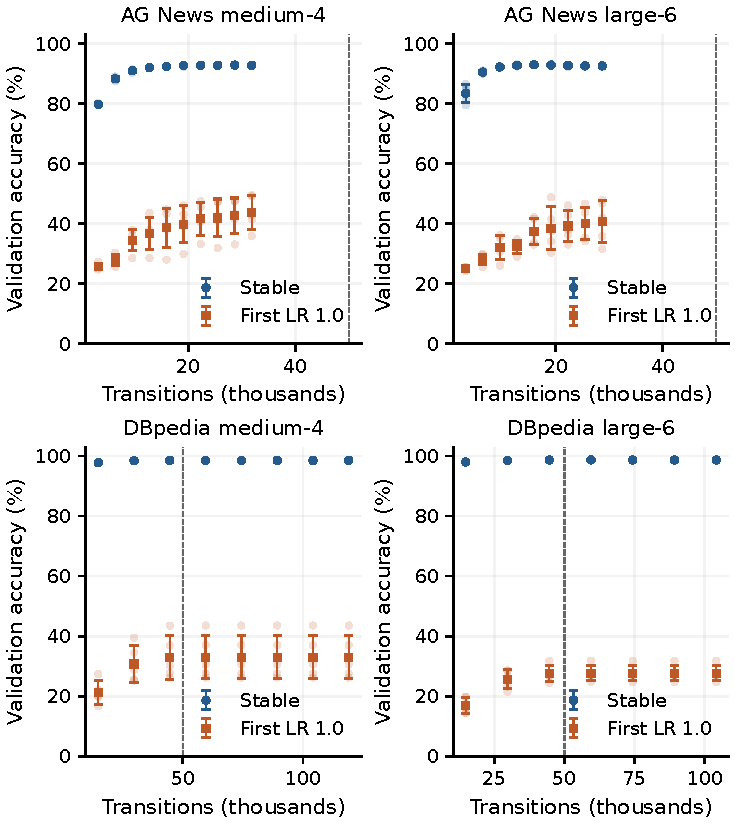
\includegraphics[width=0.97\linewidth,height=\textheight,keepaspectratio,height=0.72\textheight,keepaspectratio]{Fig1.pdf}
\caption{Validation at every step shared by both stable-family arms and all five seeds. Faint dots show individual seeds; larger markers and bars show mean and sample SD. The dashed line is the stable zero-LR boundary. Only logged observations are displayed}
\end{figure}

\begin{figure}[htbp]
\centering
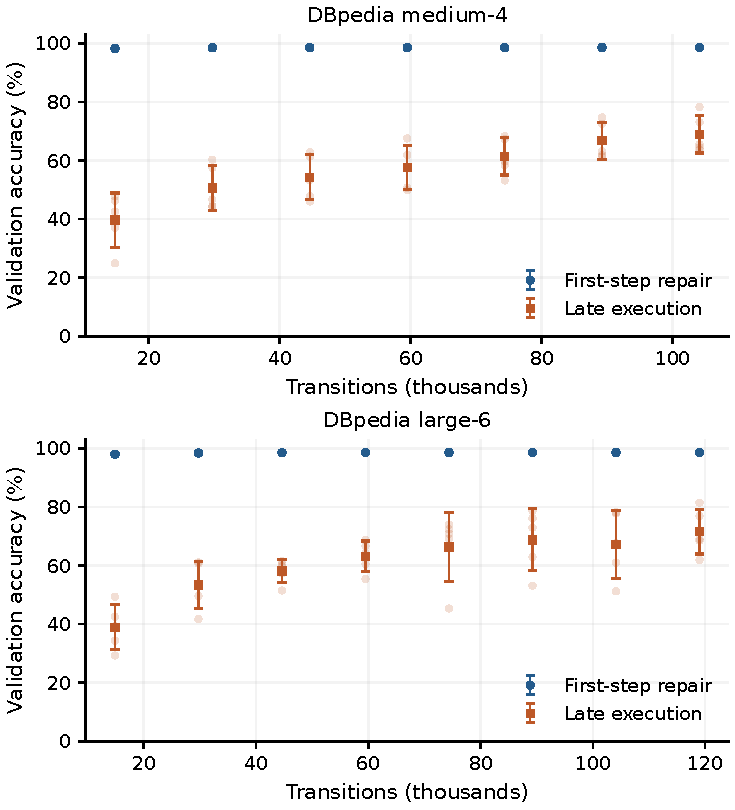
\includegraphics[width=0.97\linewidth,height=\textheight,keepaspectratio,height=0.72\textheight,keepaspectratio]{Fig2.pdf}
\caption{First-step repair while legacy lag remains: DBpedia rescue versus late execution at every step shared by both arms and all five seeds. Points and bars show mean validation accuracy and sample SD. These shared-step outcomes measure learning progress; they are not validation-selected test endpoints or equal-compute causal estimates. Complete legacy contrasts are in the supplement}
\end{figure}

\Needspace{10\baselineskip}

\textbf{Table 4. DBpedia shared-step illustration at transition 44,625.} This step is the illustration specified in the supplied plan, not a newly selected optimum. All 95 summaries are available. Shared-step validation differences and selected-test differences are distinct endpoints.

\begin{longtable}[]{@{}
  >{\raggedright\arraybackslash}p{(\linewidth - 6\tabcolsep) * \real{0.2500}}
  >{\raggedleft\arraybackslash}p{(\linewidth - 6\tabcolsep) * \real{0.2500}}
  >{\raggedleft\arraybackslash}p{(\linewidth - 6\tabcolsep) * \real{0.2500}}
  >{\raggedleft\arraybackslash}p{(\linewidth - 6\tabcolsep) * \real{0.2500}}@{}}
\toprule\noalign{}
\begin{minipage}[b]{\linewidth}\raggedright
Architecture
\end{minipage} & \begin{minipage}[b]{\linewidth}\raggedleft
Shared step
\end{minipage} & \begin{minipage}[b]{\linewidth}\raggedleft
Rescue - late validation accuracy (pp)
\end{minipage} & \begin{minipage}[b]{\linewidth}\raggedleft
Rescue - late selected test accuracy (pp)
\end{minipage} \\
\midrule\noalign{}
\endhead
\bottomrule\noalign{}
\endlastfoot
medium-4 & 44,625 & 44.293 & 5.716 \\
large-6 & 44,625 & 40.414 & 16.505 \\
\end{longtable}

The larger earlier gaps show a difference in learning progress at that step; they do not contradict the smaller selected-test gaps. They do not by themselves identify a recovery mechanism. Archived loss curves retain their batch-mean definition; DBpedia validation has full batches, while the AG News partial-batch caveat remains.

For DBpedia medium-4, comparing validation accuracy with validation accuracy gives a rescue-minus-late gap of 44.292857 percentage points at step 44,625 and 5.822619 points at the historically selected checkpoints, averaged over the same five paired seeds. The supplement lists each selected epoch and paired value. This comparison retains the original validation-loss selections; it does not reselect by accuracy or recompute predictions. The large rescue-minus-late gap concerns first-step repair while both arms retain later lag. The separate corrected-minus-rescue contrast is small and uncertain, conditional on first-step repair and the recorded stopping rules.

\subsection{Budgets and training performance}\label{budgets-and-training-performance}

The October stable cosine schedule reaches an exact zero rate for all transitions \(t\ge50{,}000\). Subsequent \texttt{optimizer.step()} calls may increment counters and consume computational resources but perform no learning-rate-dependent parameter updates for scratch Adam under these conditions (zero weight decay). The legacy inverse-square-root schedule does \textbf{not} share this terminal horizon. Inference about ``more training epochs'' therefore depends on the schedule actually assigned to the run.

Supplementary Tables S13-S14 report training performance and positive-rate, zero-rate and replay budgets separately for every condition.

The frozen schedule and logged committed early-step LRs determine the positive-LR counts. All legacy transitions remain positive; stable-family transitions at and beyond 50,000 use zero LR. The per-run supplement records the selected-checkpoint step, termination step, train metrics, cumulative LR and replay overhead. Summed LR is an exposure descriptor, not a measure of equal parameter displacement or equal effective learning. Wall-clock/GPU time is absent from these returned records and is not reconstructed from step counts. At zero LR, parameters stop moving while Adam moments and counters can still change. Selected-checkpoint and termination steps are separate fields in the per-run budget export.

All 20 DBpedia stable-family runs cross the 50,000-transition boundary. Across their stored histories, 91 consecutive pairs of validation-loss records at epochs \textbf{after} the zero boundary have exactly equal reported values; these repeated metrics cannot be interpreted as evidence of additional learning. Nine of 20 AG News stable-family runs also cross the boundary. Fourteen of the 40 stable-family runs select a best-validation epoch whose endpoint is at or beyond step 50,000, but the checkpoint can incorporate meaningful updates from \emph{before} the boundary within that epoch. Epoch-level histories alone do not identify the last useful intermediate checkpoint at precisely step 49,999. The recorded epochs therefore overstate the number of transitions available for parameter recovery.

\section{Historical severity under a distinct protocol}\label{historical-severity-under-a-distinct-protocol}

Supporting condition-level results appear in Supplementary Table S16.

Reducing the initial rate from 1.0 generally yields markedly better trained classifiers across both datasets and depths, showing that the observed failure is severity dependent rather than an all-or-nothing property of a single code branch. Differences among the smallest rates are not monotone, and this sweep does not identify a universal safe LR. The specific numerical results pertain to the historical 4,000-step warmup and three seeds; October's 8,000-step schedules, checkpoint selection records and five-seed estimates remain analytically distinct. Historical summaries use the saved notebook outcomes; prediction-level reevaluation would require the original checkpoints.

\Needspace{10\baselineskip}

\section{Pretrained generalization and monitoring distinctions}\label{pretrained-generalization-and-monitoring-distinctions}

\Needspace{10\baselineskip}

\textbf{Table 5. Pretrained primary test metrics (\%, mean \(\pm\) sample SD, five seeds).} AG News and DBpedia use macro-F1, WNUT-17 uses entity F1, and CIFAR-10 uses accuracy. Checkpoints are selected by the corresponding validation metric. Text-classification accuracy is a secondary endpoint.

\begin{longtable}[]{@{}
  >{\raggedright\arraybackslash}p{(\linewidth - 10\tabcolsep) * \real{0.1667}}
  >{\raggedleft\arraybackslash}p{(\linewidth - 10\tabcolsep) * \real{0.1667}}
  >{\raggedleft\arraybackslash}p{(\linewidth - 10\tabcolsep) * \real{0.1667}}
  >{\raggedleft\arraybackslash}p{(\linewidth - 10\tabcolsep) * \real{0.1667}}
  >{\raggedleft\arraybackslash}p{(\linewidth - 10\tabcolsep) * \real{0.1667}}
  >{\raggedright\arraybackslash}p{(\linewidth - 10\tabcolsep) * \real{0.1667}}@{}}
\toprule\noalign{}
\begin{minipage}[b]{\linewidth}\raggedright
Pretrained task
\end{minipage} & \begin{minipage}[b]{\linewidth}\raggedleft
Safe order
\end{minipage} & \begin{minipage}[b]{\linewidth}\raggedleft
Late order
\end{minipage} & \begin{minipage}[b]{\linewidth}\raggedleft
Single bad
\end{minipage} & \begin{minipage}[b]{\linewidth}\raggedleft
Guard rescue
\end{minipage} & \begin{minipage}[b]{\linewidth}\raggedright
Primary metric
\end{minipage} \\
\midrule\noalign{}
\endhead
\bottomrule\noalign{}
\endlastfoot
AG News & 94.38 \(\pm\) 0.10 & 94.38 \(\pm\) 0.08 & 94.38 \(\pm\) 0.10 & 94.40 \(\pm\) 0.09 & Macro-F1 (\%) \\
DBpedia & 99.29 \(\pm\) 0.01 & 99.29 \(\pm\) 0.01 & 99.30 \(\pm\) 0.00 & 99.29 \(\pm\) 0.02 & Macro-F1 (\%) \\
WNUT-17 & 42.28 \(\pm\) 1.56 & 42.31 \(\pm\) 1.43 & 42.49 \(\pm\) 1.34 & 42.31 \(\pm\) 1.43 & Entity F1 (\%) \\
CIFAR-10 & 96.19 \(\pm\) 0.14 & 96.11 \(\pm\) 0.17 & 96.17 \(\pm\) 0.10 & 96.16 \(\pm\) 0.18 & Accuracy (\%) \\
\end{longtable}

Pretrained results show a mismatch in the first transition and measurable displacement anomalies, but substantially smaller differences in final metrics than in the scratch configurations. The present experiment changes more than a binary ``pretrained/not pretrained'' property across studies; fault severity, optimizer, model architecture, dataset, schedule and task also differ. It does not justify concluding that pretraining \emph{caused} the smaller response.

Supporting condition-level results appear in Supplementary Table S15.

\subsection{LR assertion, displacement alarm, and downstream loss}\label{lr-assertion-displacement-alarm-and-downstream-loss}

For this known scheduling mistake, a direct assertion that the impending LR equals its intended target is the simplest prevention baseline. It stops 20/20 deliberately misordered pretrained first steps before mutation. The displacement guard is a secondary diagnostic and repair demonstration: at primary \(\kappa=10\) it detects 35/40 mismatches across eight configurations and misses all five WNUT-17 cases. These counts concern different populations, not a paired superiority test.

WNUT candidate ratios (\textasciitilde{}\(3.13\times10^{-4}\)) average about 2.05 times the fold-specific safe-window maximum, below primary thresholds near \(1.5\times10^{-3}\). This is a detection miss at that operating point, not evidence of scratch-like downstream harm. At retrospective \(\kappa=2\), all 40 mismatches exceed the threshold; that result does not prospectively validate a replacement multiplier. Zero alarms among dependent safe-window transitions do not certify a false-positive rate. Full thresholds and sensitivity are in Supplementary Table S17.

WNUT-17 reaches its peak at update 64, within the safe calibration window of updates 1-100. The reference window therefore includes peak-rate safe updates, unlike the other three pretrained tasks. This can raise the reference displacement scale relative to the first-step fault and is a possible explanation for the five misses. The records do not isolate that explanation causally; the misses should not be attributed simply to architecture or pretraining.

An LR assertion checks a specified execution invariant; displacement monitoring measures parameter motion; task metrics measure downstream utility. When the intended schedule is known and the assertion checks every parameter group immediately before mutation, it is sufficient to prevent this particular consumed-rate mismatch. Displacement adds the realized magnitude and the difference between a rejected candidate and its retained replay. It can describe an unusual update even when the rate itself is correct, but these experiments do not establish detection coverage for other fault classes. A small endpoint difference and the WNUT misses show why an alarm is neither a diagnosis of downstream harm nor a guarantee that no mismatch occurred. The current evidence does not establish general guard superiority. The guard's incremental runtime and memory overhead were not measured. The archived no-guard path also performs snapshots, so an efficiency claim would require a genuinely uninstrumented baseline.

\subsection{Replay contract and validation scope}\label{replay-contract-and-validation-scope}

Archived rescue restores weights, Adam moments/counters, parameter groups and clipped gradients, then replays the same gradient. It does not repeat the stochastic forward pass. CPU fixtures check this contract; the supplement describes finite-state checks and their limits. The new configured-peak runner separately passed an actual-device/data resume check and has no rollback intervention. Neither check certifies original-host stochastic replay or the unperformed recovery extension.

\section{Configured-peak fault at a fixed positive-LR budget}\label{configured-peak-fault-at-a-fixed-positive-lr-budget}

The extreme and configured-peak findings constrain each other's interpretation. In historical DBpedia medium-4 runs, the stable and LR=1.0 conditions have selected-test accuracies of \(98.62\pm0.02\%\) and \(33.09\pm7.20\%\) (five-seed mean and sample SD; Table 2). In the new fixed-budget pair, the corresponding test accuracies are 98.5986\% and 98.6029\% (Table 6). The historical result shows a severe deficit under its procedure; the new result shows that a much smaller first-rate error need not produce a comparable final deficit in the tested configuration. The comparison varies seed count, stopping, sampler implementation and environment, so it does not isolate fault magnitude as the sole cause of the cross-study difference.

The configured-peak first step produces a small fixed-final CE difference: validation CE is 0.061363441 for clean and 0.061368136 for peak-first, giving the prespecified contrast \(+4.695\times10^{-6}\). Validation accuracy is 98.5024\% versus 98.5107\%; test accuracy is 98.5986\% versus 98.6029\%. The accuracy differences correspond to seven additional correct validation predictions and three additional correct test predictions for peak-first. These fixed-set counts are descriptive, not evidence of a population advantage or equivalence.

\Needspace{10\baselineskip}

\textbf{Table 6. Fixed-final results for the new DBpedia medium-4 pair (seed 42).} Both arms receive 49,999 positive-LR transitions and zero zero-LR transitions. CE is uncapped and example-weighted; the training subset is not the full training population.

\begin{longtable}[]{@{}
  >{\raggedright\arraybackslash}p{(\linewidth - 8\tabcolsep) * \real{0.2000}}
  >{\raggedleft\arraybackslash}p{(\linewidth - 8\tabcolsep) * \real{0.2000}}
  >{\raggedleft\arraybackslash}p{(\linewidth - 8\tabcolsep) * \real{0.2000}}
  >{\raggedleft\arraybackslash}p{(\linewidth - 8\tabcolsep) * \real{0.2000}}
  >{\raggedleft\arraybackslash}p{(\linewidth - 8\tabcolsep) * \real{0.2000}}@{}}
\toprule\noalign{}
\begin{minipage}[b]{\linewidth}\raggedright
Population
\end{minipage} & \begin{minipage}[b]{\linewidth}\raggedleft
Clean CE
\end{minipage} & \begin{minipage}[b]{\linewidth}\raggedleft
Peak-first CE
\end{minipage} & \begin{minipage}[b]{\linewidth}\raggedleft
Clean accuracy (\%)
\end{minipage} & \begin{minipage}[b]{\linewidth}\raggedleft
Peak-first accuracy (\%)
\end{minipage} \\
\midrule\noalign{}
\endhead
\bottomrule\noalign{}
\endlastfoot
Validation (primary CE) & 0.061363441 & 0.061368136 & 98.5024 & 98.5107 \\
Official test & 0.057490380 & 0.057494741 & 98.5986 & 98.6029 \\
Fixed training subset & 0.043689493 & 0.043722571 & 99.0112 & 98.9868 \\
\end{longtable}

\begin{figure}[htbp]
\centering
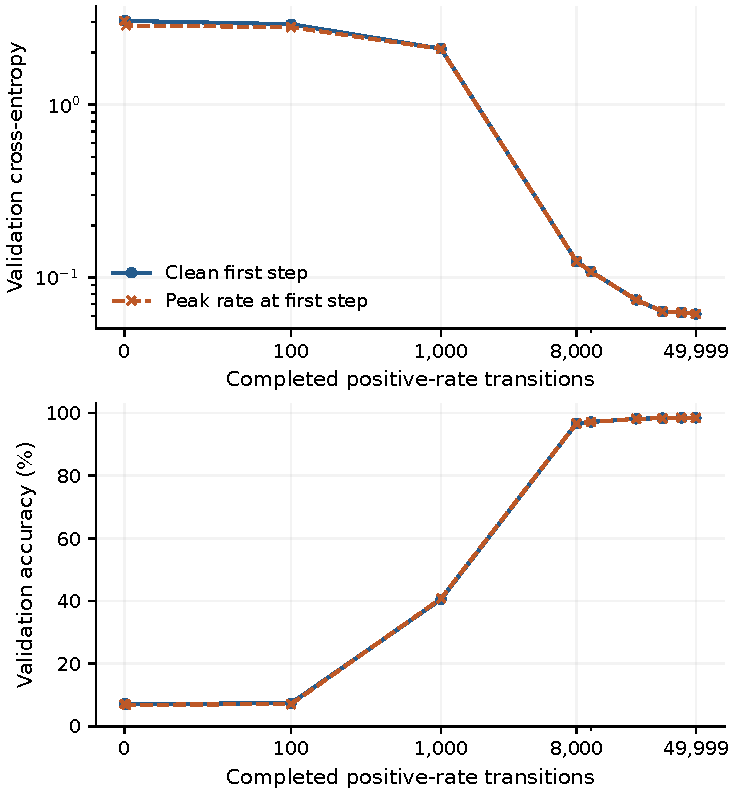
\includegraphics[width=0.98\linewidth,height=\textheight,keepaspectratio,height=0.72\textheight,keepaspectratio]{Fig3.pdf}
\caption{Absolute validation CE and accuracy at every prespecified checkpoint for the single matched pair. Both arms use the same positive-LR budget; overlapping late trajectories are retained. The horizontal scale is linear near zero and logarithmic beyond 100 transitions. No seed intervals or equivalence inference are shown}
\end{figure}

The early metrics do not support a simple damage-and-recovery narrative. Immediately after the first transition, peak-first has lower validation CE (2.872100 versus 3.051227) but lower accuracy (6.8857\% versus 7.1226\%). At transition 100 its accuracy is 0.3012 percentage points lower; at 1,000 it is 0.2440 points higher. All prespecified later contrasts are retained in the supplement. The first realized normalized displacements are \(6.604\times10^{-8}\) and \(5.066\times10^{-4}\); the saved first-step moments match while weights differ. Thus a substantially larger initial update is present without the large final task deficit seen in the extreme-fault records.

The recorded session took 82.83 minutes, including training, evaluation and checkpointing. Instrumented training time was 34.80 minutes for clean and 34.95 for peak-first; evaluation took 4.97 and 4.93 minutes. Both budgets and costs are reported separately in the supplement. These timings characterize this run, not guard overhead or an uninstrumented speed comparison.

This new within-pair comparison controls initialization, streams, schedule and fixed budget. Its tiny observed endpoint contrast narrows the practical interpretation of the historical LR=1.0 stress test. Differences in stopping, sampler implementation, hardware and software prevent treating the historical and new results as a fully controlled cross-study dose-response. A single seed and absence of a prespecified equivalence margin preclude a general safety or equivalence conclusion.

\section{Discussion and limitations}\label{discussion-and-limitations}

The experiments support a practical sequence of checks. Verify the rate immediately before the optimizer mutates state; inspect the resulting displacement; then compare validation at shared training steps and report how many positive-rate updates remain. A rate check establishes execution conformity, a displacement trace measures parameter movement, and task performance establishes the observed consequence. Substituting one for another obscures the problem: a corrected exit log can hide the first fault, a selected endpoint can hide learning delay, and extra epochs at zero rate can look like recovery training without moving the parameters.

The contrast between the severe LR=1.0 deficit and the tiny configured-peak endpoint difference restricts the practical claim. A large relative first-update displacement is not by itself evidence of a large final deficit. The new pair's early loss and accuracy contrasts also change differently, so a single crossing or favorable endpoint does not demonstrate damage followed by recovery. The recorded interventions and learning curves are observations; representation damage, curvature changes and a recovery mechanism remain untested explanations. The single new seed supplies neither an equivalence bound nor a general safe-rate threshold.

Historical selection remains part of the measured procedure. Unequal stopping and the missing legacy factorial cell prevent a complete interaction or equal-compute causal estimate. The shared-step comparisons are descriptive and preserve every common logged horizon. Five-seed intervals are unadjusted; small differences do not establish equivalence. AG News's partial validation batch may have changed historical checkpoint rankings, which cannot be recomputed without candidate-level outputs. The supplement preserves that uncertainty, the clipped-probability NLL distinction and the unavailable historical evidence.

Smaller pretrained effects cannot be attributed to pretraining alone because task, architecture, optimizer, schedule and fault magnitude differ. Depth and width also vary together. Displacement monitoring requires calibration and misses all five WNUT cases at its primary threshold; fault prevalence and guard overhead are unmeasured. A direct LR assertion is adequate for preventing the specified schedule mismatch, while displacement remains additional diagnostic evidence. We do not establish general guard superiority, permanent damage or recovery beyond the available positive-rate budget.

\section{Conclusion}\label{conclusion}

Executed learning rates, shared-step learning progress and positive-rate budgets give different information about a training failure. The recorded comparisons separate a single incorrect first update from continuing scheduler lag, show how selected endpoints can conceal substantial earlier differences, and identify when additional epochs cease to provide parameter-learning updates. The configured-peak pair's small endpoint contrast limits extrapolation from the extreme first-rate fault. The practical result is a reproducible way to interpret these particular execution failures while preserving uncertainty about mechanisms, historical selections and generalization.

\backmatter
\section*{Statements and Declarations}\label{statements-and-declarations}

\bmhead{Funding}\label{funding}

This research received no financial funding. It used resources provided by Innopolis University.

\bmhead{Competing interests}\label{competing-interests}

The authors have no relevant financial or non-financial competing interests to disclose.

\bmhead{Author contributions}\label{author-contributions}

Tivdzua Lubem Noah developed the implementation, analysed the results, and drafted and revised the manuscript. Bader Rasheed supervised the research, executed experiments, and reviewed and revised the manuscript. Dmitriy S. Vatolin contributed to the research.

\bmhead{Data and code availability}\label{data-and-code-availability}

The supplementary materials are available through the following links in the \href{https://github.com/tivdzualubem/warmup-update-budget-acml2026/tree/sncs-submission-2026-11-24}{versioned research repository} (version \texttt{sncs-submission-2026-11-24}).

\href{https://github.com/tivdzualubem/warmup-update-budget-acml2026/raw/refs/tags/sncs-submission-2026-11-24/submission/sncs-2026-11-24/ESM_1.pdf}{Online Resource 1: supplementary results and provenance} contains the complete seed-level endpoint results, recorded training trajectories, budgets, provenance and evaluation limitations.

\href{https://github.com/tivdzualubem/warmup-update-budget-acml2026/raw/refs/tags/sncs-submission-2026-11-24/submission/sncs-2026-11-24/ESM_2.zip}{Online Resource 2: reproducibility package} contains the code, configurations, retained experimental records, tests, execution logs and editable manuscript sources used to regenerate the reported tables and figures. The same files can be browsed in the repository's \texttt{sncs/} directory. Earlier experiment and rebuttal code and the previous Computing release are retained separately.

The larger prediction and retained-state archives for the configured-peak pair are stored separately and can be requested from the authors; their filenames and SHA-256 hashes are registered in the package. Historical candidate-epoch weights and matching validation predictions were not recovered and cannot be supplied. The public dataset sources are \href{https://huggingface.co/datasets/fancyzhx/ag_news}{AG News}, \href{https://huggingface.co/datasets/fancyzhx/dbpedia_14}{DBpedia}, \href{https://huggingface.co/datasets/flaitenberger/wnut_17}{WNUT-17} and \href{https://huggingface.co/datasets/uoft-cs/cifar10}{CIFAR-10}. Exact revisions, split definitions and hashes are retained in the configurations and provenance records.

%% BioMed_Central_Bib_Style_v1.01

\begin{thebibliography}{17}
% BibTex style file: bmc-mathphys.bst (version 2.1), 2014-07-24
\ifx \bisbn   \undefined \def \bisbn  #1{ISBN #1}\fi
\ifx \binits  \undefined \def \binits#1{#1}\fi
\ifx \bauthor  \undefined \def \bauthor#1{#1}\fi
\ifx \batitle  \undefined \def \batitle#1{#1}\fi
\ifx \bjtitle  \undefined \def \bjtitle#1{#1}\fi
\ifx \bvolume  \undefined \def \bvolume#1{\textbf{#1}}\fi
\ifx \byear  \undefined \def \byear#1{#1}\fi
\ifx \bissue  \undefined \def \bissue#1{#1}\fi
\ifx \bfpage  \undefined \def \bfpage#1{#1}\fi
\ifx \blpage  \undefined \def \blpage #1{#1}\fi
\ifx \burl  \undefined \def \burl#1{\textsf{#1}}\fi
\ifx \doiurl  \undefined \def \doiurl#1{\url{https://doi.org/#1}}\fi
\ifx \betal  \undefined \def \betal{\textit{et al.}}\fi
\ifx \binstitute  \undefined \def \binstitute#1{#1}\fi
\ifx \binstitutionaled  \undefined \def \binstitutionaled#1{#1}\fi
\ifx \bctitle  \undefined \def \bctitle#1{#1}\fi
\ifx \beditor  \undefined \def \beditor#1{#1}\fi
\ifx \bpublisher  \undefined \def \bpublisher#1{#1}\fi
\ifx \bbtitle  \undefined \def \bbtitle#1{#1}\fi
\ifx \bedition  \undefined \def \bedition#1{#1}\fi
\ifx \bseriesno  \undefined \def \bseriesno#1{#1}\fi
\ifx \blocation  \undefined \def \blocation#1{#1}\fi
\ifx \bsertitle  \undefined \def \bsertitle#1{#1}\fi
\ifx \bsnm \undefined \def \bsnm#1{#1}\fi
\ifx \bsuffix \undefined \def \bsuffix#1{#1}\fi
\ifx \bparticle \undefined \def \bparticle#1{#1}\fi
\ifx \barticle \undefined \def \barticle#1{#1}\fi
\bibcommenthead
\ifx \bconfdate \undefined \def \bconfdate #1{#1}\fi
\ifx \botherref \undefined \def \botherref #1{#1}\fi
\ifx \url \undefined \def \url#1{\textsf{#1}}\fi
\ifx \bchapter \undefined \def \bchapter#1{#1}\fi
\ifx \bbook \undefined \def \bbook#1{#1}\fi
\ifx \bcomment \undefined \def \bcomment#1{#1}\fi
\ifx \oauthor \undefined \def \oauthor#1{#1}\fi
\ifx \citeauthoryear \undefined \def \citeauthoryear#1{#1}\fi
\ifx \endbibitem  \undefined \def \endbibitem {}\fi
\ifx \bconflocation  \undefined \def \bconflocation#1{#1}\fi
\ifx \arxivurl  \undefined \def \arxivurl#1{\textsf{#1}}\fi
\csname PreBibitemsHook\endcsname

%%% 1
\bibitem[\protect\citeauthoryear{Gotmare et~al.}{2019}]{gotmare2019heuristics}
\begin{bchapter}
\bauthor{\bsnm{Gotmare}, \binits{A.}},
\bauthor{\bsnm{Keskar}, \binits{N.S.}},
\bauthor{\bsnm{Xiong}, \binits{C.}},
\bauthor{\bsnm{Socher}, \binits{R.}}:
\bctitle{A closer look at deep learning heuristics: Learning rate restarts,
  warmup and distillation}.
In: \bbtitle{International Conference on Learning Representations}
(\byear{2019}).
\burl{https://arxiv.org/abs/1810.13243}
\end{bchapter}
\endbibitem

%%% 2
\bibitem[\protect\citeauthoryear{Liu et~al.}{2020}]{liu2020variance}
\begin{bchapter}
\bauthor{\bsnm{Liu}, \binits{L.}},
\bauthor{\bsnm{Jiang}, \binits{H.}},
\bauthor{\bsnm{He}, \binits{P.}},
\bauthor{\bsnm{Chen}, \binits{W.}},
\bauthor{\bsnm{Liu}, \binits{X.}},
\bauthor{\bsnm{Gao}, \binits{J.}},
\bauthor{\bsnm{Han}, \binits{J.}}:
\bctitle{On the variance of the adaptive learning rate and beyond}.
In: \bbtitle{International Conference on Learning Representations}
(\byear{2020}).
\burl{https://arxiv.org/abs/1908.03265}
\end{bchapter}
\endbibitem

%%% 3
\bibitem[\protect\citeauthoryear{Ma and Yarats}{2021}]{ma2021untuned}
\begin{barticle}
\bauthor{\bsnm{Ma}, \binits{J.}},
\bauthor{\bsnm{Yarats}, \binits{D.}}:
\batitle{On the adequacy of untuned warmup for adaptive optimization}.
\bjtitle{Proceedings of the AAAI Conference on Artificial Intelligence}
\bvolume{35}(\bissue{10}),
\bfpage{8828}--\blpage{8836}
(\byear{2021})
\doiurl{10.1609/aaai.v35i10.17069}
\end{barticle}
\endbibitem

%%% 4
\bibitem[\protect\citeauthoryear{Kalra and Barkeshli}{2024}]{kalra2024warmup}
\begin{bchapter}
\bauthor{\bsnm{Kalra}, \binits{D.S.}},
\bauthor{\bsnm{Barkeshli}, \binits{M.}}:
\bctitle{Why warmup the learning rate? underlying mechanisms and improvements}.
In: \bbtitle{Advances in Neural Information Processing Systems},
vol. \bseriesno{37}
(\byear{2024}).
\doiurl{10.52202/079017-3549} .
\burl{https://proceedings.neurips.cc/paper_files/paper/2024/hash/ca98452d4e9ecbc18c40da2aa0da8b98-Abstract-Conference.html}
\end{bchapter}
\endbibitem

%%% 5
\bibitem[\protect\citeauthoryear{Abuduweili and
  Liu}{2025}]{abuduweili2025initial}
\begin{bchapter}
\bauthor{\bsnm{Abuduweili}, \binits{A.}},
\bauthor{\bsnm{Liu}, \binits{C.}}:
\bctitle{Revisiting the initial steps in adaptive gradient descent
  optimization}.
In: \bbtitle{Conference on Parsimony and Learning}.
\bsertitle{Proceedings of Machine Learning Research},
vol. \bseriesno{280},
pp. \bfpage{305}--\blpage{322}.
\bpublisher{PMLR}
(\byear{2025}).
\burl{https://proceedings.mlr.press/v280/abuduweili25a.html}
\end{bchapter}
\endbibitem

%%% 6
\bibitem[\protect\citeauthoryear{Kingma and Ba}{2015}]{kingma2015adam}
\begin{bchapter}
\bauthor{\bsnm{Kingma}, \binits{D.P.}},
\bauthor{\bsnm{Ba}, \binits{J.}}:
\bctitle{{Adam}: A method for stochastic optimization}.
In: \bbtitle{International Conference on Learning Representations}
(\byear{2015}).
\burl{https://arxiv.org/abs/1412.6980}
\end{bchapter}
\endbibitem

%%% 7
\bibitem[\protect\citeauthoryear{Shazeer and
  Stern}{2018}]{shazeer2018adafactor}
\begin{bchapter}
\bauthor{\bsnm{Shazeer}, \binits{N.}},
\bauthor{\bsnm{Stern}, \binits{M.}}:
\bctitle{Adafactor: Adaptive learning rates with sublinear memory cost}.
In: \bbtitle{Proceedings of the 35th International Conference on Machine
  Learning}.
\bsertitle{Proceedings of Machine Learning Research},
vol. \bseriesno{80},
pp. \bfpage{4596}--\blpage{4604}.
\bpublisher{PMLR}
(\byear{2018}).
\burl{https://proceedings.mlr.press/v80/shazeer18a.html}
\end{bchapter}
\endbibitem

%%% 8
\bibitem[\protect\citeauthoryear{Kosson et~al.}{2024}]{kosson2024warmup}
\begin{bchapter}
\bauthor{\bsnm{Kosson}, \binits{A.}},
\bauthor{\bsnm{Messmer}, \binits{B.}},
\bauthor{\bsnm{Jaggi}, \binits{M.}}:
\bctitle{Analyzing \& reducing the need for learning rate warmup in {GPT}
  training}.
In: \bbtitle{Advances in Neural Information Processing Systems},
vol. \bseriesno{37}
(\byear{2024}).
\doiurl{10.52202/079017-0096} .
\burl{https://proceedings.neurips.cc/paper_files/paper/2024/hash/059445c2d5b3ef918079851628fef1d6-Abstract-Conference.html}
\end{bchapter}
\endbibitem

%%% 9
\bibitem[\protect\citeauthoryear{Ben~Braiek and
  Khomh}{2023}]{benbraiek2023deepchecker}
\begin{barticle}
\bauthor{\bsnm{Ben~Braiek}, \binits{H.}},
\bauthor{\bsnm{Khomh}, \binits{F.}}:
\batitle{Testing feedforward neural networks training programs}.
\bjtitle{ACM Transactions on Software Engineering and Methodology}
\bvolume{32}(\bissue{4}),
\bfpage{1}--\blpage{61}
(\byear{2023})
\doiurl{10.1145/3529318}
\end{barticle}
\endbibitem

%%% 10
\bibitem[\protect\citeauthoryear{Wardat et~al.}{2022}]{wardat2022deepdiagnosis}
\begin{bchapter}
\bauthor{\bsnm{Wardat}, \binits{M.}},
\bauthor{\bsnm{Cruz}, \binits{B.D.}},
\bauthor{\bsnm{Le}, \binits{W.}},
\bauthor{\bsnm{Rajan}, \binits{H.}}:
\bctitle{{DeepDiagnosis}: Automatically diagnosing faults and recommending
  actionable fixes in deep learning programs}.
In: \bbtitle{Proceedings of the 44th International Conference on Software
  Engineering},
pp. \bfpage{561}--\blpage{572}.
\bpublisher{ACM}
(\byear{2022}).
\doiurl{10.1145/3510003.3510071} .
\burl{https://doi.org/10.1145/3510003.3510071}
\end{bchapter}
\endbibitem

%%% 11
\bibitem[\protect\citeauthoryear{Bai et~al.}{2026}]{bai2026spikes}
\begin{bchapter}
\bauthor{\bsnm{Bai}, \binits{Z.}},
\bauthor{\bsnm{Zhou}, \binits{Z.}},
\bauthor{\bsnm{Zhao}, \binits{J.}},
\bauthor{\bsnm{Li}, \binits{X.}},
\bauthor{\bsnm{Li}, \binits{Z.}},
\bauthor{\bsnm{Xiong}, \binits{F.}},
\bauthor{\bsnm{Yang}, \binits{H.}},
\bauthor{\bsnm{Zhang}, \binits{Y.}},
\bauthor{\bsnm{Xu}, \binits{Z.-Q.J.}}:
\bctitle{Adaptive preconditioners trigger loss spikes in {Adam}}.
In: \bbtitle{Proceedings of the 43rd International Conference on Machine
  Learning}.
\bsertitle{Proceedings of Machine Learning Research},
vol. \bseriesno{306},
pp. \bfpage{5566}--\blpage{5601}.
\bpublisher{PMLR}
(\byear{2026}).
\burl{https://proceedings.mlr.press/v306/bai26o.html}
\end{bchapter}
\endbibitem

%%% 12
\bibitem[\protect\citeauthoryear{Alimisis et~al.}{2026}]{alimisis2026warmup}
\begin{bchapter}
\bauthor{\bsnm{Alimisis}, \binits{F.}},
\bauthor{\bsnm{Islamov}, \binits{R.}},
\bauthor{\bsnm{Lucchi}, \binits{A.}}:
\bctitle{Why do we need warm-up? {A} theoretical perspective}.
In: \bbtitle{Proceedings of the 43rd International Conference on Machine
  Learning}.
\bsertitle{Proceedings of Machine Learning Research},
vol. \bseriesno{306},
pp. \bfpage{1909}--\blpage{1980}.
\bpublisher{PMLR}
(\byear{2026}).
\burl{https://proceedings.mlr.press/v306/alimisis26a.html}
\end{bchapter}
\endbibitem

%%% 13
\bibitem[\protect\citeauthoryear{Guo et~al.}{2017}]{guo2017calibration}
\begin{bchapter}
\bauthor{\bsnm{Guo}, \binits{C.}},
\bauthor{\bsnm{Pleiss}, \binits{G.}},
\bauthor{\bsnm{Sun}, \binits{Y.}},
\bauthor{\bsnm{Weinberger}, \binits{K.Q.}}:
\bctitle{On calibration of modern neural networks}.
In: \bbtitle{Proceedings of the 34th International Conference on Machine
  Learning}.
\bsertitle{Proceedings of Machine Learning Research},
vol. \bseriesno{70},
pp. \bfpage{1321}--\blpage{1330}.
\bpublisher{PMLR}
(\byear{2017}).
\burl{https://proceedings.mlr.press/v70/guo17a.html}
\end{bchapter}
\endbibitem

%%% 14
\bibitem[\protect\citeauthoryear{Vaswani et~al.}{2017}]{vaswani2017attention}
\begin{bchapter}
\bauthor{\bsnm{Vaswani}, \binits{A.}},
\bauthor{\bsnm{Shazeer}, \binits{N.}},
\bauthor{\bsnm{Parmar}, \binits{N.}},
\bauthor{\bsnm{Uszkoreit}, \binits{J.}},
\bauthor{\bsnm{Jones}, \binits{L.}},
\bauthor{\bsnm{Gomez}, \binits{A.N.}},
\bauthor{\bsnm{Kaiser}, \binits{{\L}.}},
\bauthor{\bsnm{Polosukhin}, \binits{I.}}:
\bctitle{Attention is all you need}.
In: \bbtitle{Advances in Neural Information Processing Systems},
vol. \bseriesno{30}
(\byear{2017}).
\burl{https://proceedings.neurips.cc/paper/2017/hash/3f5ee243547dee91fbd053c1c4a845aa-Abstract.html}
\end{bchapter}
\endbibitem

%%% 15
\bibitem[\protect\citeauthoryear{Huang et~al.}{2020}]{huang2020initialization}
\begin{bchapter}
\bauthor{\bsnm{Huang}, \binits{X.S.}},
\bauthor{\bsnm{Perez}, \binits{F.}},
\bauthor{\bsnm{Ba}, \binits{J.}},
\bauthor{\bsnm{Volkovs}, \binits{M.}}:
\bctitle{Improving {Transformer} optimization through better initialization}.
In: \bbtitle{Proceedings of the 37th International Conference on Machine
  Learning}.
\bsertitle{Proceedings of Machine Learning Research},
vol. \bseriesno{119},
pp. \bfpage{4475}--\blpage{4483}.
\bpublisher{PMLR}
(\byear{2020}).
\burl{https://proceedings.mlr.press/v119/huang20f.html}
\end{bchapter}
\endbibitem

%%% 16
\bibitem[\protect\citeauthoryear{Xiong et~al.}{2020}]{xiong2020layernorm}
\begin{bchapter}
\bauthor{\bsnm{Xiong}, \binits{R.}},
\bauthor{\bsnm{Yang}, \binits{Y.}},
\bauthor{\bsnm{He}, \binits{D.}},
\bauthor{\bsnm{Zheng}, \binits{K.}},
\bauthor{\bsnm{Zheng}, \binits{S.}},
\bauthor{\bsnm{Xing}, \binits{C.}},
\bauthor{\bsnm{Zhang}, \binits{H.}},
\bauthor{\bsnm{Lan}, \binits{Y.}},
\bauthor{\bsnm{Wang}, \binits{L.}},
\bauthor{\bsnm{Liu}, \binits{T.}}:
\bctitle{On layer normalization in the {Transformer} architecture}.
In: \bbtitle{Proceedings of the 37th International Conference on Machine
  Learning}.
\bsertitle{Proceedings of Machine Learning Research},
vol. \bseriesno{119},
pp. \bfpage{10524}--\blpage{10533}.
\bpublisher{PMLR}
(\byear{2020}).
\burl{https://proceedings.mlr.press/v119/xiong20b.html}
\end{bchapter}
\endbibitem

%%% 17
\bibitem[\protect\citeauthoryear{Loshchilov and
  Hutter}{2019}]{loshchilov2019decoupled}
\begin{bchapter}
\bauthor{\bsnm{Loshchilov}, \binits{I.}},
\bauthor{\bsnm{Hutter}, \binits{F.}}:
\bctitle{Decoupled weight decay regularization}.
In: \bbtitle{International Conference on Learning Representations}
(\byear{2019}).
\burl{https://arxiv.org/abs/1711.05101}
\end{bchapter}
\endbibitem

\end{thebibliography}

\end{document}
